\subsection{Glyph: \glyph{Not}}
\label{sec:af:not}

The glyph \glyph{not} is used to denote that the \glyph{AFN} linked as input cannot produce the output.

\begin{glyphDescription}
 \glyphSboTerm SBO:0000238 ! not.
 \glyphOrigin One AFN (section~\ref{sec:af:AFNs}) or logical operator (section~\ref{sec:af:logic}).
 \glyphTarget
 \glyphNode \glyph{Not} is represented by a circle carrying the word ``NOT''.
 \end{glyphDescription}

\begin{figure}[H]
  \centering
  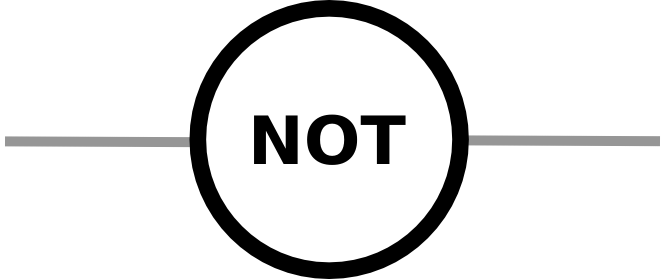
\includegraphics[scale = 0.5]{images/not}
  \caption{The \AF glyph for \glyph{not}.}
  \label{fig:af:not}
\end{figure}
